\documentclass[12pt]{article}
\usepackage[utf8]{inputenc}
\usepackage[english]{babel}
\usepackage{amsmath, amssymb, amsthm, bm}
\usepackage{geometry}
\usepackage{tikz}
\usetikzlibrary{shapes, backgrounds, positioning, arrows.meta, calc, fit}
\usepackage{caption}
\usepackage{setspace}
\usepackage{enumitem}
\usepackage{booktabs}
%\usepackage[backend=biber,style=chicago-authordate]{biblatex}

\usepackage[round]{natbib}

% Hyperref for clickable Table of Contents and citations
\usepackage{hyperref}
\hypersetup{
	colorlinks=true,
	linkcolor=blue,
	filecolor=magenta,      
	urlcolor=cyan,
	citecolor=red,
}

% Custom theorem styles
\newtheorem{theorem}{Theorem}[section]
\newtheorem{lemma}[theorem]{Lemma}
\newtheorem{definition}{Definition}[section]
\newtheorem{example}{Example}[section]
\newtheorem{proposition}{Proposition}[section]

\geometry{letterpaper, margin=1in}
\onehalfspacing

\begin{document}
	
	\title{\textbf{Mathematical Definition and Equivalence Proof: \\ The Tool Switching Problem and the Generalized Traveling Salesman Problem}}
	\author{Shankar Narayanan \\ \textit{Internship Report} \\ \textit{Advisors: Prof. Rafael Colares and Prof. Annegret Wagler}}
	\date{March 30, 2026}
	
	\maketitle
	
	\begin{abstract}
		The management of tool configurations in Flexible Manufacturing Systems (FMS) is a well-studied combinatorial optimization challenge. Because tool switches consume valuable production time, minimizing these operations is a critical objective. This report provides a mathematical analysis of the Standard Tool Switching Problem (SSP). We explore a non-compact, configuration-based integer programming formulation that eradicates the symmetry issues plaguing traditional models. A primary contribution of this work is the proof of equivalence between the proposed SSP formulation and the Generalized Traveling Salesman Problem (GTSP). Building upon this equivalence, we propose an advanced, exact Branch-and-Price algorithmic pathway. By surveying state-of-the-art literature, we outline an experimental roadmap to accelerate the exact pricing oracle utilizing Machine Learning techniques such as Deep Reinforcement Learning for diverse column selection and Regression for objective bound prediction.
	\end{abstract}
	
	\newpage
	
	\section{Introduction}
	
	Flexible Manufacturing Systems (FMS) enable rapid adaptation to market changes by utilizing numerically controlled machines equipped with automated tool magazines. Because a single machine may be required to process a diverse batch of parts, and because the total number of distinct tools required often exceeds the capacity of the machine's magazine, tool switches are unavoidable \citep{Tang1988}. A tool switch incurs a time penalty that delays production. Consequently, optimal tool management is a primary objective in operations research.
	
	The literature broadly divides tool management into two distinct problems based on operational constraints:
	\begin{enumerate}
		\item \textbf{The Job Grouping Problem (JGP):} Occurs when a machine must be entirely stopped to change tools, allowing multiple tools to be swapped simultaneously. The objective is to partition the jobs into a minimum number of feasible groups, effectively treating the issue as a Set Covering problem \citep{Crama1994}.
		\item \textbf{The Tool Switching Problem (SSP):} Models environments where jobs are processed sequentially and tool switches occur individually. The objective is to simultaneously determine the optimal job processing sequence and the tool loading policy to minimize the total number of individual tool switches \citep{Catanzaro2015}.
	\end{enumerate}
	
	This report focuses exclusively on the latter: the sequential Tool Switching Problem (SSP). We aim to formalize the mathematical properties of a non-compact formulation that models the SSP as a routing problem over valid tool configurations. By proving its equivalence to the Generalized Traveling Salesman Problem (GTSP), we establish an exact framework capable of exploiting both decades of highly optimized routing heuristics and modern Artificial Intelligence approaches for dynamic graph generation.
	
	
	\section{The Colares-Wagler Non-Compact Formulation}
	
	
	The computational complexity of the SSP is fundamentally rooted in its state space. Traditional compact models sequence the jobs directly and track tool insertions step-by-step. However, these models suffer from extreme symmetry caused by \textit{0-blocks}---intervals where a tool is retained in the magazine across multiple jobs despite not being required, forcing the solver to evaluate highly symmetric, redundant permutations \citep{Catanzaro2015, Laporte2004}. 
	
	To establish an intuitive foundation before introducing the formal mathematics, consider the small instance illustrated in Figure \ref{fig:incidence_matrix}. 
	
	\begin{figure}[h!]
		\centering
		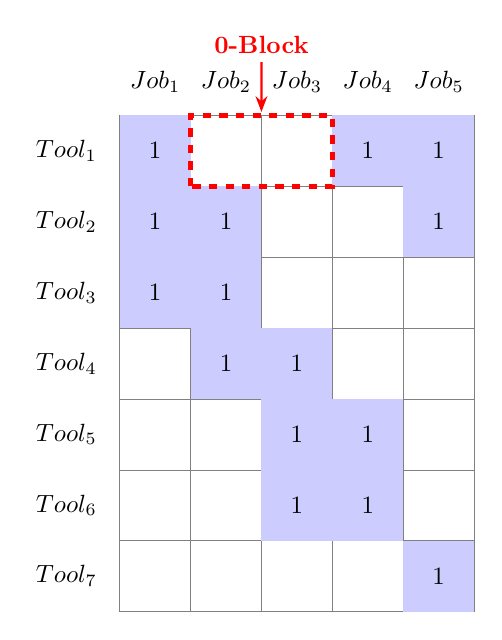
\begin{tikzpicture}[scale=0.9, every node/.style={transform shape}]
			% Grid
			\draw[step=1cm,gray,very thin] (0,0) grid (5,7);
			
			% Row labels (Tools)
			\node[font=\bfseries, anchor=east] at (-0.2, 6.5) {$Tool_1$};
			\node[font=\bfseries, anchor=east] at (-0.2, 5.5) {$Tool_2$};
			\node[font=\bfseries, anchor=east] at (-0.2, 4.5) {$Tool_3$};
			\node[font=\bfseries, anchor=east] at (-0.2, 3.5) {$Tool_4$};
			\node[font=\bfseries, anchor=east] at (-0.2, 2.5) {$Tool_5$};
			\node[font=\bfseries, anchor=east] at (-0.2, 1.5) {$Tool_6$};
			\node[font=\bfseries, anchor=east] at (-0.2, 0.5) {$Tool_7$};
			
			% Col labels (Jobs)
			\node[font=\bfseries, anchor=south] at (0.5, 7.2) {$Job_1$};
			\node[font=\bfseries, anchor=south] at (1.5, 7.2) {$Job_2$};
			\node[font=\bfseries, anchor=south] at (2.5, 7.2) {$Job_3$};
			\node[font=\bfseries, anchor=south] at (3.5, 7.2) {$Job_4$};
			\node[font=\bfseries, anchor=south] at (4.5, 7.2) {$Job_5$};
			
			% Fill required tools 
			% Job 1: 1, 2, 3
			\fill[blue!20] (0,6) rectangle (1,7); \node at (0.5, 6.5) {1};
			\fill[blue!20] (0,5) rectangle (1,6); \node at (0.5, 5.5) {1};
			\fill[blue!20] (0,4) rectangle (1,5); \node at (0.5, 4.5) {1};
			
			% Job 2: 2, 3, 4
			\fill[blue!20] (1,5) rectangle (2,6); \node at (1.5, 5.5) {1};
			\fill[blue!20] (1,4) rectangle (2,5); \node at (1.5, 4.5) {1};
			\fill[blue!20] (1,3) rectangle (2,4); \node at (1.5, 3.5) {1};
			
			% Job 3: 4, 5, 6
			\fill[blue!20] (2,3) rectangle (3,4); \node at (2.5, 3.5) {1};
			\fill[blue!20] (2,2) rectangle (3,3); \node at (2.5, 2.5) {1};
			\fill[blue!20] (2,1) rectangle (3,2); \node at (2.5, 1.5) {1};
			
			% Job 4: 1, 5, 6
			\fill[blue!20] (3,6) rectangle (4,7); \node at (3.5, 6.5) {1};
			\fill[blue!20] (3,2) rectangle (4,3); \node at (3.5, 2.5) {1};
			\fill[blue!20] (3,1) rectangle (4,2); \node at (3.5, 1.5) {1};
			
			% Job 5: 1, 2, 7
			\fill[blue!20] (4,6) rectangle (5,7); \node at (4.5, 6.5) {1};
			\fill[blue!20] (4,5) rectangle (5,6); \node at (4.5, 5.5) {1};
			\fill[blue!20] (4,0) rectangle (5,1); \node at (4.5, 0.5) {1};
			
			% Highlight 0-block for Tool 1 across Job 2 and 3 (Fixed Overlap)
			\draw[red, ultra thick, dashed] (1,6) rectangle (3,7);
			\node[red, font=\bfseries] (0block) at (2, 8.0) {0-Block};
			\draw[red, thick, -{Stealth[length=2mm]}] (0block) -- (2, 7.05);
			
		\end{tikzpicture}
		\caption{An incidence matrix for a 5-job, 7-tool instance. The machine magazine has a capacity $b=4$. Assuming the sequence $1 \to 2 \to 3 \to 4 \to 5$, Tool 1 is required by Jobs 1, 4, and 5. Because $b=4$ is large enough to accommodate the transition tool requirements without ejecting Tool 1, it can be retained through Jobs 2 and 3. This retention interval is known as a 0-block, as it avoids redundant unloading and reloading operations.}
		\label{fig:incidence_matrix}
	\end{figure}
	
	\subsection{Illustrative Example: Magazine State Evolution}
	
	To illustrate the tool switching mechanics and the concrete impact of a 0-block, consider the 5-job, 7-tool instance previously introduced in Figure \ref{fig:incidence_matrix}. The machine has a magazine capacity of $b=4$, and the jobs are processed in the sequence $j_1 \to j_2 \to j_3 \to j_4 \to j_5$. The specific tool requirements for each job are as follows:
	\begin{itemize}
		\item $T_1 = \{t_1, t_2, t_3\}$
		\item $T_2 = \{t_2, t_3, t_4\}$
		\item $T_3 = \{t_4, t_5, t_6\}$
		\item $T_4 = \{t_1, t_5, t_6\}$
		\item $T_5 = \{t_1, t_2, t_7\}$
	\end{itemize}
	
	Under the optimal Keep Tool Needed Soonest (KTNS) policy \citep{Tang1988}, the solver looks ahead to minimize future swaps. The evolution of the optimal magazine configurations across this sequence is depicted in Figure \ref{fig:magazine_timeline}.
	
	\begin{figure}[h!]
		\centering
		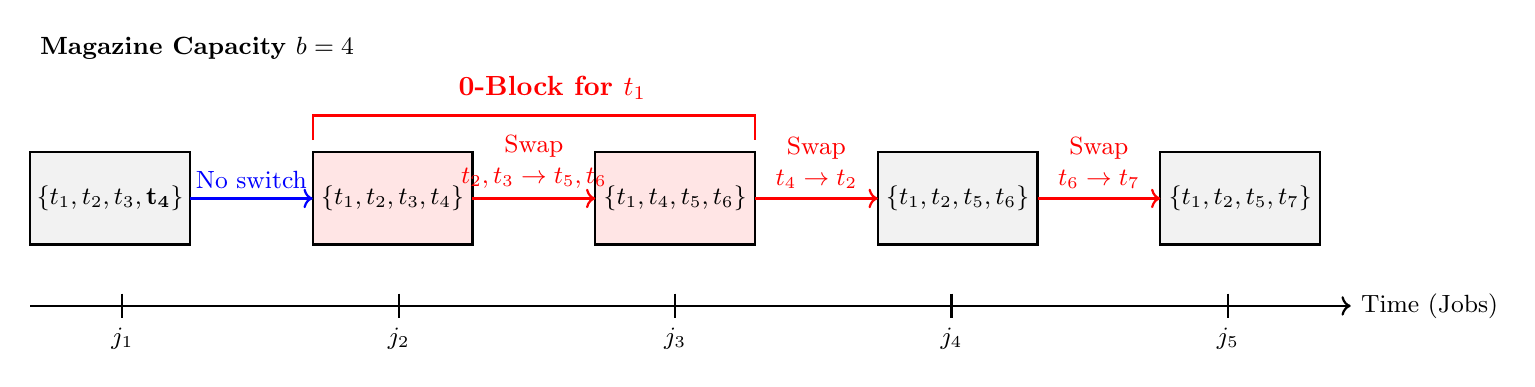
\begin{tikzpicture}[scale=0.78, every node/.style={font=\small}]
			% Time Axis
			\draw[->, thick] (-0.5,0) -- (21,0) node[right] {Time (Jobs)};
			
			% Job Markers
			\foreach \x/\t in {1/j_1, 5.5/j_2, 10/j_3, 14.5/j_4, 19/j_5} {
				\draw[thick] (\x, 0.2) -- (\x, -0.2) node[below] {$\t$};
			}
			
			% Magazine Slots (Configurations)
			\draw[thick, fill=gray!10] (-0.5,1) rectangle (2.1,2.5) node[midway] {$\{t_1, t_2, t_3, \mathbf{t_4}\}$};
			\draw[thick, fill=red!10] (4.1,1) rectangle (6.7,2.5) node[midway] {$\{t_1, t_2, t_3, t_4\}$};
			\draw[thick, fill=red!10] (8.7,1) rectangle (11.3,2.5) node[midway] {$\{t_1, t_4, t_5, t_6\}$};
			\draw[thick, fill=gray!10] (13.3,1) rectangle (15.9,2.5) node[midway] {$\{t_1, t_2, t_5, t_6\}$};
			\draw[thick, fill=gray!10] (17.9,1) rectangle (20.5,2.5) node[midway] {$\{t_1, t_2, t_5, t_7\}$};
			
			% Switch Indicators
			\draw[->, blue, thick] (2.1, 1.75) -- (4.1, 1.75) node[midway, above] {No switch};
			\draw[->, red, thick] (6.7, 1.75) -- (8.7, 1.75) node[midway, above, align=center] {Swap \\ $t_2, t_3 \to t_5, t_6$};
			\draw[->, red, thick] (11.3, 1.75) -- (13.3, 1.75) node[midway, above, align=center] {Swap \\ $t_4 \to t_2$};
			\draw[->, red, thick] (15.9, 1.75) -- (17.9, 1.75) node[midway, above, align=center] {Swap \\ $t_6 \to t_7$};
			
			% 0-Block Highlight (Manual bracket for safe compilation)
			\draw[thick, red] (4.1, 2.7) -- (4.1, 3.1) -- (11.3, 3.1) -- (11.3, 2.7);
			\node[red, font=\bfseries, above] at (8, 3.2) {0-Block for $t_1$};
			
			\node[anchor=west] at (-0.5,4.2) {\textbf{Magazine Capacity $b=4$}};
		\end{tikzpicture}
		\caption{State-space timeline of the tool magazine. Because tool $t_4$ is required for $j_2$, it is preemptively loaded in the free slot during $j_1$, preventing a switch. Most importantly, tool $t_1$ is required for jobs $j_1$ and $j_4$, but not for $j_2$ and $j_3$. Because the magazine capacity is large enough to accommodate the transition tools without evicting $t_1$, it is safely retained across the 0-block, avoiding redundant unloading and reloading operations.}
		\label{fig:magazine_timeline}
	\end{figure}
	
	To bypass the sequence-based symmetry inherent in tracking such 0-blocks step-by-step, we utilize the non-compact formulation proposed by \citet{Colares2026}, which projects the problem entirely onto a complete directed graph of valid configurations.
	
	\subsection{Definitions, Variables, and Maximal Configurations}
	Let $J = \{1, 2, \dots, n\}$ be the set of jobs and $T = \{1, 2, \dots, m\}$ be the set of all available tools. Each job $j \in J$ requires a specific subset of tools $T_j \subseteq T$. The machine's tool magazine has a capacity $b$. 
	
	A fundamental property of this formulation is the assumption of \textit{maximal configurations}. Let $\mathcal{C} = \{C \subseteq T \mid |C| \le b\}$ be the collection of all valid tool configurations. Without loss of generality, we establish that the tool repository is always full, i.e., $|C| = b$ for all considered configurations \citep{Colares2026}. 
	
	\begin{proposition}[Configuration Maximization]
		Any configuration $C$ where $|C| < b$ is strictly dominated by a maximal configuration $C' = C \cup T_{dummy}$ where $|C'| = b$.
	\end{proposition}
	\begin{proof}
		Let $d(C_1, C_2)$ be the number of tool switches required to transition from configuration $C_1$ to $C_2$. The cost formula evaluates to $d(C_1, C_2) = b - |C_1 \cap C_2|$. If $|C_1| < b$, the empty slots can be filled with arbitrary tools from $T \setminus C_1$ to form $C_1'$, yielding $|C_1'| = b$. Because $C_1 \subseteq C_1'$, it mathematically follows that $|C_1 \cap C_2| \le |C_1' \cap C_2|$. Therefore, $b - |C_1' \cap C_2| \le b - |C_1 \cap C_2|$. Padding an under-capacity configuration incurs a mathematical penalty of zero while strictly increasing the probability that the added tools may satisfy subsequent job requirements, thereby avoiding future switches \citep{Tang1988}. Thus, we can safely assume $|C| = b$ for all $C \in \mathcal{C}$.
	\end{proof}
	
	We consider the complete graph $K_p$, where each vertex $v \in V(K_p)$ corresponds to a distinct maximal configuration $C \in \mathcal{C}$. The edge weight $d(u,v)$ represents the number of tool switches required to transition from configuration $C_u$ to $C_v$:
	\begin{equation}
		d(u,v) = b - |C_u \cap C_v|
	\end{equation}
	Let $H_j \subseteq V(K_p)$ denote the subset of configurations capable of processing job $j \in J$ (i.e., $T_j \subseteq C$). The formulation utilizes two binary decision variables: $y(v) \in \{0, 1\}$ indicating whether configuration $v$ is used to process some job, and $x(u,v) \in \{0, 1\}$ indicating whether configuration $v$ is applied right after configuration $u$ in the sequence.
	
	\subsection{Mathematical Model and Correctness}
	The non-compact SSP is formulated over the complete graph $K_p$ as follows:
	\begin{align}
		\min \quad & \sum_{u \in V(K_p)} \sum_{v \in V(K_p)} d(u,v) x(u,v) \label{eq:nc_obj} \\
		\text{s.t.} \quad & \sum_{v \in H_j} y(v) \ge 1 && \forall j \in J \label{eq:nc_cover} \\
		& \sum_{u \in V(K_p)} x(u,v) = y(v) && \forall v \in V(K_p) \label{eq:nc_flowin} \\
		& \sum_{u \in V(K_p)} x(v,u) = y(v) && \forall v \in V(K_p) \label{eq:nc_flowout} \\
		& \sum_{u \in H(S)} \sum_{v \in H(S)} x(u,v) \le \sum_{v \in H(S)} y(v) - 1 && \forall S \subseteq J, \ 2 \le |S| \le |J| - 1 \label{eq:nc_sec} \\
		& x(u,v) \in \{0, 1\} && \forall u, v \in V(K_p) \label{eq:nc_varx} \\
		& y(v) \in \{0, 1\} && \forall v \in V(K_p) \label{eq:nc_vary}
	\end{align}
	where $H(S) = \bigcup_{j \in S} H_j$.
	
	To establish the correctness of this formulation, we must prove that the constraints mathematically enforce a valid, continuous sequence of configurations that covers all jobs, and that the objective evaluates the optimal tool switching cost without loss of generality.
	
	\begin{lemma}[Flow and Cover Feasibility]
		Constraints \eqref{eq:nc_cover}, \eqref{eq:nc_flowin}, and \eqref{eq:nc_flowout} ensure that the active configurations ($y(v) = 1$) form a collection of node-disjoint directed cycles such that every job $j \in J$ is covered by at least one active configuration.
	\end{lemma}
	\begin{proof}
		By constraint \eqref{eq:nc_cover}, for every $j \in J$, there exists at least one configuration $v \in H_j$ such that $y(v) \ge 1$. Since $y(v) \in \{0,1\}$, this forces $y(v) = 1$. Constraints \eqref{eq:nc_flowin} and \eqref{eq:nc_flowout} are flow conservation equations. They dictate that if a configuration $v$ is active ($y(v)=1$), it must have exactly one incoming edge and one outgoing edge. If $y(v)=0$, it has no incident edges. In any finite directed graph, a subgraph where every active vertex has an in-degree and out-degree of exactly 1 inherently decomposes into a set of node-disjoint directed cycles. Therefore, the active configurations form a set of closed cycles that collectively cover all job tool requirements.
	\end{proof}
	
	\begin{lemma}[Subtour Elimination]
		Constraint \eqref{eq:nc_sec} guarantees that the active configurations form exactly one connected Hamiltonian cycle.
	\end{lemma}
	\begin{proof}
		Suppose, for the sake of contradiction, that a feasible solution satisfying \eqref{eq:nc_cover}--\eqref{eq:nc_flowout} forms $k \ge 2$ disjoint directed cycles, $W_1, W_2, \dots, W_k$. Let $V(W_1)$ be the set of active vertices in cycle $W_1$. Let $S \subset J$ be the proper subset of jobs covered exclusively by the configurations in $W_1$. Because $k \ge 2$ and the clusters $H_j$ partition the job requirements, $W_1$ cannot process all jobs without rendering the other cycles completely redundant. Thus, $2 \le |S| \le |J|-1$. 
		
		By definition, all vertices in $W_1$ belong to $H(S) = \bigcup_{j \in S} H_j$, meaning $V(W_1) \subseteq H(S)$. If we sum the selected edges $x(u,v)$ within $W_1$, we have:
		\begin{equation}
			\sum_{u \in V(W_1)} \sum_{v \in V(W_1)} x(u,v) = |V(W_1)| = \sum_{v \in V(W_1)} y(v)
		\end{equation}
		Since $V(W_1) \subseteq H(S)$, evaluating the Subtour Elimination Constraint \eqref{eq:nc_sec} strictly over $S$ yields:
		\begin{equation}
			\sum_{u \in H(S)} \sum_{v \in H(S)} x(u,v) \ge \sum_{v \in V(W_1)} y(v)
		\end{equation}
		However, constraint \eqref{eq:nc_sec} strictly bounds the sum of the edges from above, demanding $\sum_{u \in H(S)} \sum_{v \in H(S)} x(u,v) \le \sum_{v \in H(S)} y(v) - 1$. This constitutes a direct contradiction. Thus, the formulation strictly forbids disjoint sub-cycles, enforcing $k=1$.
	\end{proof}
	
	\begin{theorem}[Correctness]
		The integer linear program defined by \eqref{eq:nc_obj}--\eqref{eq:nc_vary} correctly identifies an optimal job sequence and tool-loading policy that minimizes the total number of tool switches for the SSP.
	\end{theorem}
	\begin{proof}
		By Lemma 2.1 and Lemma 2.2, the formulation's constraints define a single, connected cycle over a subset of configuration vertices that collectively satisfy all job requirements. For any two consecutively applied configurations $C_u$ and $C_v$ (where $x(u,v)=1$), the number of tools that must be inserted into the magazine is exactly the capacity $b$ minus the number of tools retained from the previous configuration, $|C_u \cap C_v|$. Thus, the transition edge cost $d(u,v) = b - |C_u \cap C_v|$ exactly computes the number of physical tool switches required. The objective function \eqref{eq:nc_obj} accumulates these transition costs along the active edges of the cycle. Therefore, minimizing this objective over the feasible space correctly yields a sequence mapping directly to the absolute minimum number of tool switches.
	\end{proof}
	
	\section{Equivalence Between the SSP and the GTSP}
	
	To bridge the Tool Switching Problem (SSP) with the Generalized Traveling Salesman Problem (GTSP), we must mathematically establish a two-way reduction. We will demonstrate that the configuration-based SSP maps to the GTSP via an exponential transformation, while the GTSP maps to the SSP via a polynomial transformation, proving that the SSP is a strictly harder generalization.
	
	\subsection{Formal Definition of Instances}
	We formally define an instance of the sequential SSP as $\mathcal{I}_{SSP} = \langle J, T, b, \{T_j\}_{j \in J} \rangle$, where $J = \{1, \dots, n\}$ is the set of jobs, $T = \{1, \dots, m\}$ is the set of tools, $b$ is the magazine capacity, and $T_j \subseteq T$ is the tool requirement for job $j$. The input size of this problem is bounded by $\mathcal{O}(|J| \cdot |T|)$. 
	
	We define an instance of the GTSP using standard graph notation as $\mathcal{I}_{GTSP} = \langle V, E, d, \{V_k\}_{k \in K} \rangle$. Here, $V$ is the set of vertices, $E$ is the set of edges with a distance function $d : E \to \mathbb{R}^+$, and $K = \{1, \dots, k\}$ is an index set for the clusters. The collection $\{V_k\}_{k \in K}$ is a partition of $V$ into $k$ mutually exclusive, disjoint clusters such that $V_p \cap V_q = \emptyset$ for all $p \neq q$ \citep{Pop2024}.
	
	\subsection{Reduction 1: SSP to GTSP (Forward Mapping)}
	
	In the SSP, a single maximal tool configuration $C \in \mathcal{C}$ can contain the necessary tools to satisfy multiple jobs simultaneously. Therefore, the configuration clusters $H_j$ are inherently overlapping ($H_i \cap H_j \neq \emptyset$). To map this to the GTSP, we adapt the Intersecting-to-Nonintersecting (I-N) transformation \citep{Lien1993, Noon1993}.
	
	\textbf{The Construction:} We construct the GTSP vertex set $V$ by duplicating valid SSP configurations into job-specific replicas:
	\begin{equation}
		V = \{ v_{C, j} \mid C \in \mathcal{C}, \ j \in J, \ T_j \subseteq C \}
	\end{equation}
	The vertices are partitioned into exactly $|J|$ clusters. Each cluster $V_j$ corresponds uniquely to a job $j \in J$:
	\begin{equation}
		V_j = \{ v_{C, j} \mid C \in \mathcal{C}, \ T_j \subseteq C \} \quad \forall j \in J
	\end{equation}
	Because each replica vertex is uniquely indexed by its job $j$, the clusters are strictly disjoint ($V_i \cap V_j = \emptyset$). The distance function $d$ between any two replicas in $V$ is defined as the number of tool switches required to transition between their underlying configurations:
	\begin{equation}
		d(v_{C_1, i}, v_{C_2, j}) = b - |C_1 \cap C_2|
	\end{equation}
	
	\begin{lemma}[Triangular Inequality]
		The transition distance function $d(u,v) = b - |C_u \cap C_v|$ satisfies the triangular inequality.
	\end{lemma}
	\begin{proof}
		Let $C_1, C_2, C_3$ be any three maximal configurations such that $|C_i| = b$. We must show $d(v_1, v_3) \le d(v_1, v_2) + d(v_2, v_3)$, which translates to:
		\begin{equation}
			b - |C_1 \cap C_3| \le (b - |C_1 \cap C_2|) + (b - |C_2 \cap C_3|)
		\end{equation}
		This simplifies to $|C_1 \cap C_2| + |C_2 \cap C_3| - b \le |C_1 \cap C_3|$. By basic set theory, we know that $|C_1 \cap C_2| + |C_2 \cap C_3| = |(C_1 \cap C_2) \cup (C_2 \cap C_3)| + |C_1 \cap C_2 \cap C_3|$. Since the union $(C_1 \cap C_2) \cup (C_2 \cap C_3)$ is strictly a subset of $C_2$, its size is bounded by $|C_2| = b$. Furthermore, the intersection $C_1 \cap C_2 \cap C_3$ is strictly a subset of $C_1 \cap C_3$. Therefore, $|C_1 \cap C_2| + |C_2 \cap C_3| \le b + |C_1 \cap C_3|$. Subtracting $b$ from both sides yields the required inequality.
	\end{proof}
	
	\begin{lemma}[Non-Redundant Subtours]
		If a GTSP tour visits two replicas of the same configuration non-consecutively, it can be transformed into a non-redundant tour of equal or strictly lesser cost where all replicas of that configuration are visited consecutively \citep{Lien1993}.
	\end{lemma}
	\begin{proof}
		Let $v_{C, i}$ and $v_{C, j}$ be replicas of the same configuration $C$ visited non-consecutively in a tour $T$. The distance between them is $d(v_{C,i}, v_{C,j}) = b - |C \cap C| = 0$. Because the distance matrix satisfies the triangular inequality (Lemma 3.1), bypassing intermediate nodes to visit $v_{C, j}$ immediately after $v_{C, i}$ via the zero-cost edge will never increase the total cost of the tour. Repeated application of this shortcutting procedure groups all replicas of $C$ into a continuous zero-cost subtour, yielding a non-redundant tour $T^*$ such that $Cost(T^*) \le Cost(T)$.
	\end{proof}
	
	\begin{theorem}[Bijective Cost Correspondence]
		A minimum-cost GTSP tour on the transformed graph corresponds bijectively to an optimal SSP sequence without loss of optimality.
	\end{theorem}
	\begin{proof}
		By Lemma 3.2, there always exists an optimal GTSP tour that is non-redundant. In a non-redundant tour, all replicas of a chosen configuration $C$ are visited consecutively, incurring an internal transition cost of $0$ between them. This perfectly emulates the Keep Tool Needed Soonest (KTNS) policy, which retains tool configurations across a 0-block of jobs at zero penalty \citep{Catanzaro2015}. Consequently, this non-redundant sequence of disjoint clusters collapses directly into a valid, sequence-preserving tool-loading policy for the SSP with identical cost.
	\end{proof}
	
	\begin{figure}[h!]
		\centering
		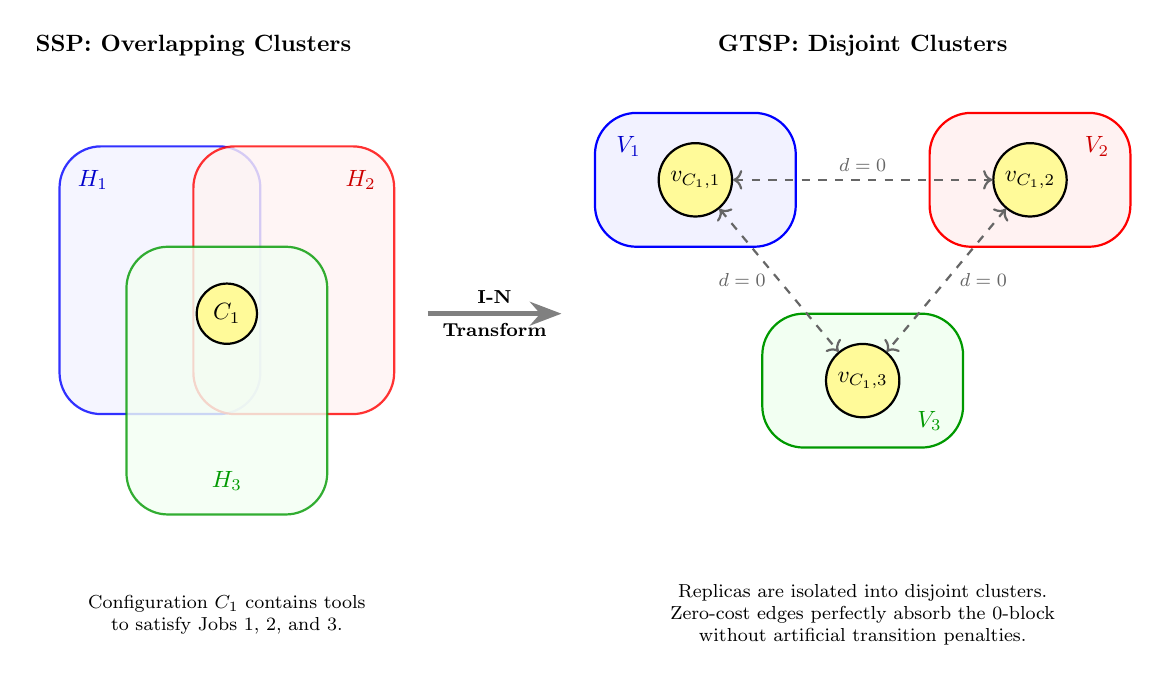
\begin{tikzpicture}[scale=0.85, every node/.style={transform shape}]
			
			% SSP Side
			\node[font=\bfseries] at (2, 5.5) {SSP: Overlapping Clusters};
			
			\draw[thick, blue, fill=blue!5, rounded corners=15pt, opacity=0.8] (0, 0) rectangle (3, 4);
			\node[blue!80!black, font=\bfseries] at (0.5, 3.5) {$H_{1}$};
			
			\draw[thick, red, fill=red!5, rounded corners=15pt, opacity=0.8] (2, 0) rectangle (5, 4);
			\node[red!80!black, font=\bfseries] at (4.5, 3.5) {$H_{2}$};
			
			\draw[thick, green!60!black, fill=green!5, rounded corners=15pt, opacity=0.8] (1, -1.5) rectangle (4, 2.5);
			\node[green!60!black, font=\bfseries] at (2.5, -1) {$H_{3}$};
			
			\node[draw, circle, fill=yellow!40, thick, minimum size=0.9cm] (C1) at (2.5, 1.5) {$C_1$};
			
			\node[align=center, font=\footnotesize, text width=4.5cm] at (2.5, -3) {Configuration $C_1$ contains tools \\ to satisfy Jobs 1, 2, and 3.};
			
			% Arrow
			\draw[-{Stealth[length=4mm]}, line width=2pt, gray] (5.5, 1.5) -- (7.5, 1.5) 
			node[midway, above, font=\footnotesize\bfseries, text=black] {I-N} 
			node[midway, below, font=\footnotesize\bfseries, text=black] {Transform};
			
			% GTSP Side
			\node[font=\bfseries] at (12, 5.5) {GTSP: Disjoint Clusters};
			
			\draw[thick, blue, fill=blue!5, rounded corners=15pt] (8, 2.5) rectangle (11, 4.5);
			\node[blue!80!black, font=\bfseries] at (8.5, 4) {$V_{1}$};
			\node[draw, circle, fill=yellow!40, thick, minimum size=0.8cm] (v1) at (9.5, 3.5) {$v_{C_1, 1}$};
			
			\draw[thick, red, fill=red!5, rounded corners=15pt] (13, 2.5) rectangle (16, 4.5);
			\node[red!80!black, font=\bfseries] at (15.5, 4) {$V_{2}$};
			\node[draw, circle, fill=yellow!40, thick, minimum size=0.8cm] (v2) at (14.5, 3.5) {$v_{C_1, 2}$};
			
			\draw[thick, green!60!black, fill=green!5, rounded corners=15pt] (10.5, -0.5) rectangle (13.5, 1.5);
			\node[green!60!black, font=\bfseries] at (13, -0.1) {$V_{3}$};
			\node[draw, circle, fill=yellow!40, thick, minimum size=0.8cm] (v3) at (12, 0.5) {$v_{C_1, 3}$};
			
			% Zero Cost Edges
			\draw[<->, thick, dashed, gray!80!black] (v1) -- (v2) node[midway, above, font=\footnotesize\bfseries] {$d = 0$};
			\draw[<->, thick, dashed, gray!80!black] (v1) -- (v3) node[midway, left, font=\footnotesize\bfseries, xshift=-2pt] {$d = 0$};
			\draw[<->, thick, dashed, gray!80!black] (v2) -- (v3) node[midway, right, font=\footnotesize\bfseries, xshift=2pt] {$d = 0$};
			
			\node[align=center, font=\footnotesize, text width=6cm] at (12, -3) {Replicas are isolated into disjoint clusters. \\ Zero-cost edges perfectly absorb the 0-block \\ without artificial transition penalties.};
			
		\end{tikzpicture}
		\caption{Forward Mapping (SSP $\rightarrow$ GTSP). A single configuration $C_1$ covering three jobs is duplicated into mutually exclusive replicas connected by zero-cost edges, establishing a bijective mapping to the optimal SSP tool retention logic.}
		\label{fig:forward_mapping}
	\end{figure}
	
	\subsection{Reduction 2: GTSP to SSP (Reverse Mapping)}
	
	To prove that the SSP is a strictly harder generalization, we must demonstrate that any arbitrary GTSP instance can be polynomially reduced to an SSP instance under a strict \textit{Disjointness Condition}. 
	
	\textbf{The Construction:} Given an arbitrary GTSP instance $\mathcal{I}_{GTSP} = \langle V, E, d, \{V_k\}_{k \in K} \rangle$, we construct an SSP instance $\mathcal{I}_{SSP}$ as follows:
	\begin{enumerate}
		\item \textbf{Jobs and Capacity:} Let the set of jobs $J = K = \{1, 2, \dots, k\}$. Set the magazine capacity $b = \max_{p=1}^k |V_p|$.
		\item \textbf{Tool Padding:} Let every vertex $v \in V$ become a unique tool. To prevent any single configuration of size $b$ from inadvertently covering multiple smaller clusters, we must enforce uniform tool requirements. For each cluster $V_p$, we generate a set of distinct dummy tools $D_p$ such that $|V_p \cup D_p| = b$. 
		\item \textbf{Tool Set:} The complete tool repository is $T = V \cup (\bigcup_{p=1}^k D_p)$.
		\item \textbf{Job Requirements:} For each job $p \in J$, define its tool requirement as $T_p = V_p \cup D_p$.
	\end{enumerate}
	
	\begin{lemma}[Strict Disjointness]
		The dummy-tool padding algorithm guarantees that no two jobs can share any tools in the constructed SSP instance, forcing $|T_p \cup T_q| = 2b > b$ for all $p \neq q$.
	\end{lemma}
	\begin{proof}
		In the original GTSP, clusters are mutually exclusive by definition, meaning $V_p \cap V_q = \emptyset$ for all $p \neq q$. During the padding step, the dummy tools $D_p$ are generated uniquely for each job, implying $D_p \cap D_q = \emptyset$ and $D_p \cap V = \emptyset$. Therefore, the padded tool requirements $T_p = V_p \cup D_p$ and $T_q = V_q \cup D_q$ must satisfy strict mutual exclusivity: $T_p \cap T_q = \emptyset$. Consequently, the union of any two distinct job requirements evaluates strictly to $|T_p \cup T_q| = |T_p| + |T_q| = b + b = 2b$. Because $2b > b$, the capacity constraint is strictly violated for any union of job requirements.
	\end{proof}
	
	\begin{theorem}[Polynomial Reduction and Equivalence]
		Any arbitrary instance of the GTSP can be polynomially reduced to an instance of the SSP. 
	\end{theorem}
	\begin{proof}
		By Lemma 3.3, the constructed SSP enforces a Strict Disjointness Condition. Because no valid tool configuration $C$ can exceed the capacity bound ($|C| \le b$), it is physically impossible for any single tool configuration to contain the tools to process more than one job. This mathematically enforces $H_p \cap H_q = \emptyset$ for all $p \neq q$. The configuration clusters in the constructed SSP are structurally forced to be disjoint, effectively collapsing the overlapping mechanics of the SSP directly back into a standard GTSP. The reduction creates exactly $k$ jobs, sets capacity $b \le |V|$, and defines $|T| \le k \cdot |V|$ tools. Thus, the transformation is strictly bounded by $\mathcal{O}(k \cdot |V|)$, which is polynomial.
	\end{proof}
	
	\begin{figure}[h!]
		\centering
		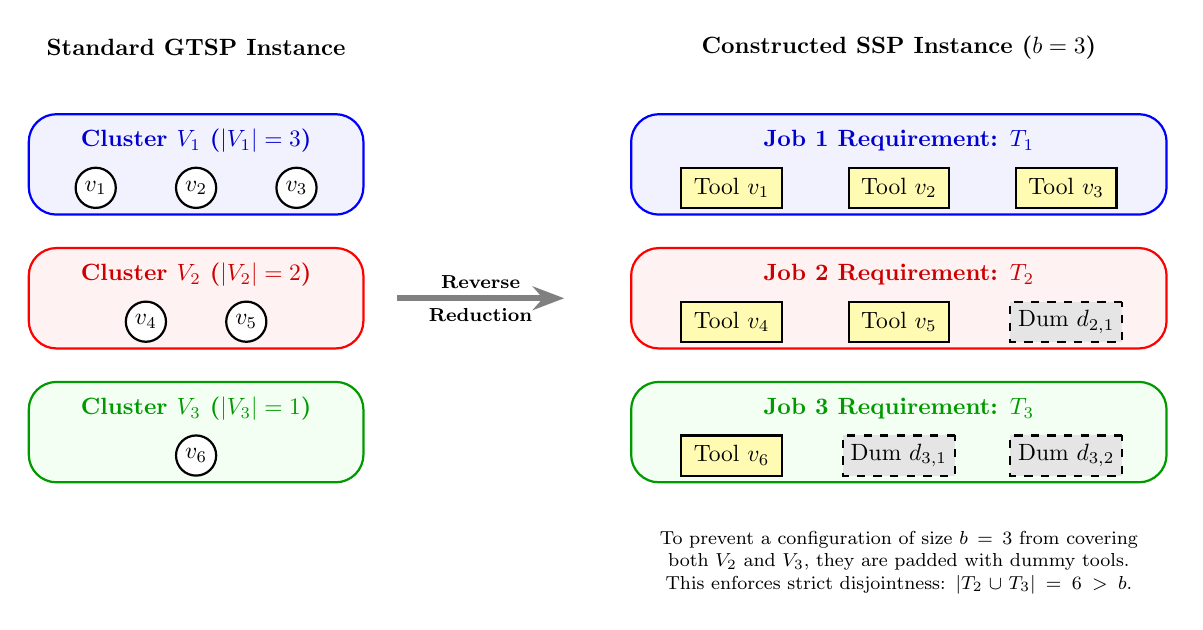
\begin{tikzpicture}[scale=0.85, every node/.style={transform shape}]
			
			% GTSP Side
			\node[font=\bfseries] at (2, 5.5) {Standard GTSP Instance};
			
			\draw[thick, blue, fill=blue!5, rounded corners=10pt] (-0.5, 3) rectangle (4.5, 4.5);
			\node[blue!80!black, font=\bfseries] at (2, 4.1) {Cluster $V_1$ ($|V_1| = 3$)};
			\node[draw, circle, fill=white, thick, minimum size=0.6cm, inner sep=1pt] (v1) at (0.5, 3.4) {$v_1$};
			\node[draw, circle, fill=white, thick, minimum size=0.6cm, inner sep=1pt] (v2) at (2, 3.4) {$v_2$};
			\node[draw, circle, fill=white, thick, minimum size=0.6cm, inner sep=1pt] (v3) at (3.5, 3.4) {$v_3$};
			
			\draw[thick, red, fill=red!5, rounded corners=10pt] (-0.5, 1) rectangle (4.5, 2.5);
			\node[red!80!black, font=\bfseries] at (2, 2.1) {Cluster $V_2$ ($|V_2| = 2$)};
			\node[draw, circle, fill=white, thick, minimum size=0.6cm, inner sep=1pt] (v4) at (1.25, 1.4) {$v_4$};
			\node[draw, circle, fill=white, thick, minimum size=0.6cm, inner sep=1pt] (v5) at (2.75, 1.4) {$v_5$};
			
			\draw[thick, green!60!black, fill=green!5, rounded corners=10pt] (-0.5, -1) rectangle (4.5, 0.5);
			\node[green!60!black, font=\bfseries] at (2, 0.1) {Cluster $V_3$ ($|V_3| = 1$)};
			\node[draw, circle, fill=white, thick, minimum size=0.6cm, inner sep=1pt] (v6) at (2, -0.6) {$v_6$};
			
			% Arrow
			\draw[-{Stealth[length=4mm]}, line width=2pt, gray] (5, 1.75) -- (7.5, 1.75) 
			node[midway, above, font=\footnotesize\bfseries, text=black] {Reverse} 
			node[midway, below, font=\footnotesize\bfseries, text=black] {Reduction};
			
			% SSP Side
			\node[font=\bfseries] at (12.5, 5.5) {Constructed SSP Instance ($b=3$)};
			
			\draw[thick, blue, fill=blue!5, rounded corners=10pt] (8.5, 3) rectangle (16.5, 4.5);
			\node[blue!80!black, font=\bfseries] at (12.5, 4.1) {Job 1 Requirement: $T_1$};
			\node[draw, rectangle, fill=yellow!30, thick, minimum height=0.6cm, minimum width=1.5cm] (t1) at (10, 3.4) {Tool $v_1$};
			\node[draw, rectangle, fill=yellow!30, thick, minimum height=0.6cm, minimum width=1.5cm] (t2) at (12.5, 3.4) {Tool $v_2$};
			\node[draw, rectangle, fill=yellow!30, thick, minimum height=0.6cm, minimum width=1.5cm] (t3) at (15, 3.4) {Tool $v_3$};
			
			\draw[thick, red, fill=red!5, rounded corners=10pt] (8.5, 1) rectangle (16.5, 2.5);
			\node[red!80!black, font=\bfseries] at (12.5, 2.1) {Job 2 Requirement: $T_2$};
			\node[draw, rectangle, fill=yellow!30, thick, minimum height=0.6cm, minimum width=1.5cm] (t4) at (10, 1.4) {Tool $v_4$};
			\node[draw, rectangle, fill=yellow!30, thick, minimum height=0.6cm, minimum width=1.5cm] (t5) at (12.5, 1.4) {Tool $v_5$};
			\node[draw, rectangle, fill=gray!20, dashed, thick, minimum height=0.6cm, minimum width=1.5cm] (d21) at (15, 1.4) {Dum $d_{2,1}$};
			
			\draw[thick, green!60!black, fill=green!5, rounded corners=10pt] (8.5, -1) rectangle (16.5, 0.5);
			\node[green!60!black, font=\bfseries] at (12.5, 0.1) {Job 3 Requirement: $T_3$};
			\node[draw, rectangle, fill=yellow!30, thick, minimum height=0.6cm, minimum width=1.5cm] (t6) at (10, -0.6) {Tool $v_6$};
			\node[draw, rectangle, fill=gray!20, dashed, thick, minimum height=0.6cm, minimum width=1.5cm] (d31) at (12.5, -0.6) {Dum $d_{3,1}$};
			\node[draw, rectangle, fill=gray!20, dashed, thick, minimum height=0.6cm, minimum width=1.5cm] (d32) at (15, -0.6) {Dum $d_{3,2}$};
			
			\node[align=center, font=\footnotesize, text width=8cm] at (12.5, -2.2) {To prevent a configuration of size $b=3$ from covering both $V_2$ and $V_3$, they are padded with dummy tools. \\ This enforces strict disjointness: $|T_2 \cup T_3| = 6 > b$.};
			
		\end{tikzpicture}
		\caption{Reverse Mapping (GTSP $\rightarrow$ SSP). Dummy tools enforce the Disjointness Condition, ensuring that no single valid tool configuration can cover multiple jobs, collapsing the SSP back into a GTSP.}
		\label{fig:reverse_reduction}
	\end{figure}
	
	\subsection{Algorithmic Implications of the Complexity Space}
	
	Because the reverse reduction is polynomial while the forward reduction is exponential, the complete configuration graph cannot always be instantiated in memory. This inherent complexity difference dictates a bifurcated solution methodology (illustrated in Figure \ref{fig:complexity_flowchart}). 
	
	For smaller instances where the capacity $b$ is restrictive, the entire GTSP graph can be generated, allowing polynomial transformations \citep{Noon1993} to convert the problem into an Asymmetric TSP solvable by highly optimized routing heuristics. However, for massive instances where $\binom{|T|}{b}$ triggers out-of-memory failures, exactness requires dynamic node generation via Branch-and-Price, utilizing advanced learning strategies to navigate the exponential state space.
	
	\begin{figure}[h!]
		\centering
		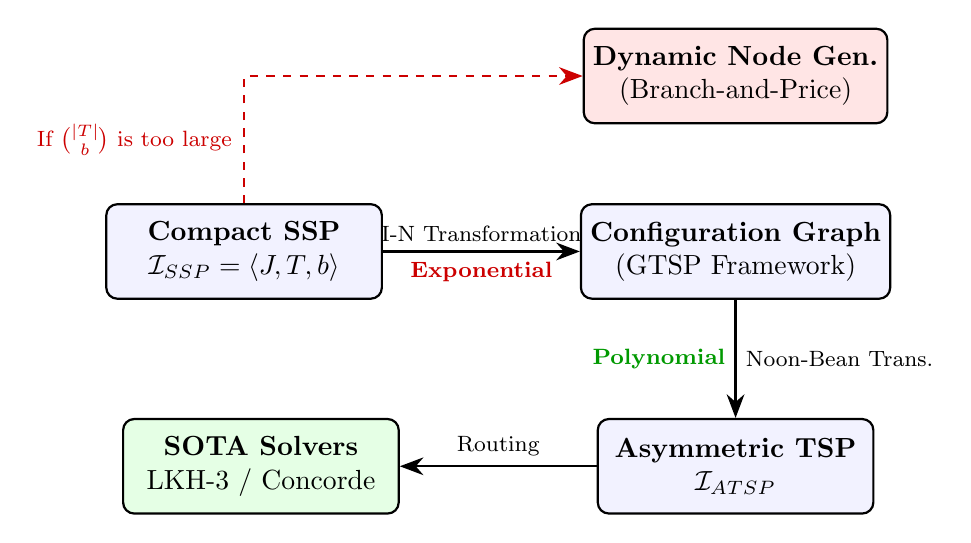
\begin{tikzpicture}[
			node distance=1.5cm and 2.5cm,
			box/.style={draw, rectangle, rounded corners, minimum width=3.5cm, minimum height=1.2cm, align=center, fill=blue!5, thick},
			arrow/.style={-{Stealth[length=3mm]}, thick}
			]
			
			% Nodes
			\node[box] (ssp) {\textbf{Compact SSP} \\ $\mathcal{I}_{SSP} = \langle J, T, b \rangle$};
			
			\node[box, right=of ssp] (gtsp) {\textbf{Configuration Graph} \\ (GTSP Framework)};
			
			\node[box, below=of gtsp] (atsp) {\textbf{Asymmetric TSP} \\ $\mathcal{I}_{ATSP}$};
			
			\node[box, fill=green!10, left=of atsp] (solvers) {\textbf{SOTA Solvers} \\ LKH-3 / Concorde};
			
			\node[box, fill=red!10, above=of gtsp, yshift=-0.5cm] (bp) {\textbf{Dynamic Node Gen.} \\ (Branch-and-Price)};
			
			% Arrows
			\draw[arrow] (ssp) -- node[above, font=\footnotesize] {I-N Transformation} node[below, font=\footnotesize\bfseries, text=red!80!black] {Exponential} (gtsp);
			
			\draw[arrow] (gtsp) -- node[right, font=\footnotesize] {Noon-Bean Trans.} node[left, font=\footnotesize\bfseries, text=green!60!black] {Polynomial} (atsp);
			
			\draw[arrow] (atsp) -- node[above, font=\footnotesize] {Routing} (solvers);
			
			\draw[arrow, dashed, red!80!black] (ssp) |- node[near start, left, font=\footnotesize, text width=2.5cm] {If $\binom{|T|}{b}$ is too large} (bp);
%			\draw[arrow, dashed, red!80!black] (bp) -- node[right, font=\footnotesize] {On-the-fly Generation} (gtsp);
			
		\end{tikzpicture}
		\caption{The complexity space of solving the SSP. Tractable instances can be reduced to ATSP and solved via highly optimized routing heuristics, while massive instances bypass the exponential bottleneck via dynamic node generation in a Branch-and-Price framework.}
		\label{fig:complexity_flowchart}
	\end{figure}
	
	
	\section{Exact Routing for Tractable Instances}
	
	For small-to-medium manufacturing environments, the total number of tools $|T|$ and the magazine capacity $b$ restrict the configuration space $|\mathcal{C}| = \binom{|T|}{b}$ to a computationally manageable size. Under these conditions, the theoretical equivalence established in Section 3 allows us to explicitly instantiate the complete graph $K_p$ and entirely bypass the complex pricing subproblems of Integer Linear Programming (ILP) solvers.
	
	\subsection{The Noon-Bean Transformation}
	When the configuration space is tractable, the complete GTSP graph and its mutually exclusive clusters $\{V_k\}_{k \in K}$ can be generated in memory. We then apply the Noon-Bean transformation \citep{Noon1993}, a graph transformation that modifies the edge weights to compel any optimal routing algorithm to visit exactly one node per cluster before moving to the next.
	
	This transformation collapses the generalized problem into a standard Asymmetric Traveling Salesman Problem (ATSP) over a directed graph. The resulting ATSP perfectly encodes the 0-block tool switching mechanics via its transition weights $d(u,v) = b - |C_u \cap C_v|$ without the sequence-based symmetry that paralyzes compact models.
	
	\subsection{Highly Optimized Routing Solvers}
	The reduction to an ATSP unlocks the application of the most powerful routing engines developed in the operations research community. The transformed graph can be fed directly into the Lin-Kernighan-Helsgaun (LKH-3) algorithm \citep{Helsgaun2015}. LKH-3 utilizes advanced $k$-opt sequential exchanges and minimum spanning tree approximations to find optimal or near-optimal tours for asymmetric instances in fractions of a second. For environments requiring a mathematically proven global optimum, the ATSP can be solved using exact branch-and-cut solvers such as Concorde \citep{Applegate2006}. 
	
	This pathway demonstrates the immediate practical superiority of the non-compact formulation: tractable SSP instances can be translated directly into the domain of pure routing, solving in seconds what traditional compact models fail to solve in hours.
	
	\section{Dynamic Node Generation and the True Pricing Bottleneck}
	
	While the reduction to ATSP is definitive for small instances, it faces a hard mathematical limit in large-scale industrial settings. As the tool repository $|T|$ and magazine capacity $b$ grow, the number of valid maximal configurations $\binom{|T|}{b}$ explodes exponentially. Generating the complete graph triggers severe out-of-memory failures. To maintain exactness without explicitly instantiating $V(K_p)$, the problem must be solved dynamically using a Branch-and-Price (B\&P) framework \citep{Barnhart1998}.
	
	\subsection{The Restricted Master Problem}
	In the B\&P framework, the algorithm initializes a \textit{Restricted Master Problem} (RMP) containing only a tiny, feasible subset of configuration nodes $V' \subset V(K_p)$. The linear relaxation of the RMP is solved to obtain dual variables associated with both the job-covering constraints \eqref{eq:nc_cover} and the flow-conservation routing constraints \eqref{eq:nc_flowin}--\eqref{eq:nc_flowout}.
	
	To prove global optimality or find improving configurations, these dual variables are passed to a Pricing Subproblem (PSP) oracle. The oracle's task is to identify a new configuration node $v \notin V'$ that possesses a negative reduced cost, meaning its addition to the RMP will improve the objective bound. 
	
	\subsection{The Complexity of the SSP Pricing Oracle}
	It is critical to formally distinguish the pricing complexity of the Tool Switching Problem (SSP) from that of the simpler Job Grouping Problem (JGP). In the JGP, the objective is purely a Set Covering task; the processing order of the configurations does not matter. Consequently, the JGP pricing oracle only needs to maximize the sum of the covering duals subject to the magazine capacity $b$. This task is formally equivalent to the Set Union Knapsack Problem (SUKP) \citep{Crama1994, Goldschmidt1994}, which, while NP-hard, can often be solved efficiently in practice.
	
	However, the non-compact SSP formulation is a simultaneous covering \textit{and sequencing} problem. Because it maps to the GTSP, the cost of a configuration heavily depends on the transition edge weights $d(u,v)$ required to travel to and from that configuration in the sequence. Therefore, the reduced cost of a new configuration node in the SSP is not just a function of its internal tools (the knapsack component); it is an explicit function of its optimal insertion point in the current routing sequence, evaluated against the routing dual variables.
	
	\begin{proposition}[NP-Hardness of the SSP Pricing Oracle]
		The exact Pricing Subproblem for the non-compact SSP is strictly harder than the SUKP, as it must simultaneously determine the optimal subset of tools to satisfy the capacity $b$ while computing the shortest transition paths from the existing nodes in the RMP to minimize the routing reduced cost.
	\end{proposition}
	\begin{proof}
		Let $\pi_j$ be the dual variables associated with the covering constraints \eqref{eq:nc_cover}, and $\gamma_v^{in}, \gamma_v^{out}$ be the dual variables associated with the flow conservation constraints \eqref{eq:nc_flowin} and \eqref{eq:nc_flowout}. The reduced cost $\bar{c}_v$ of a new configuration $v$ representing a tool set $C_v$ requires finding an incoming edge from some $u \in V'$ and an outgoing edge to some $w \in V'$ such that:
		\begin{equation}
			\bar{c}_v = \min_{u,w \in V'} \Big( d(u,v) + d(v,w) - \gamma_u^{out} - \gamma_w^{in} \Big) - \sum_{j \in J : T_j \subseteq C_v} \pi_j < 0
		\end{equation}
		Evaluating this exact oracle requires searching the exponentially large space of valid tool configurations $\mathcal{C}$ to simultaneously maximize the covered duals $\pi_j$ (the SUKP dimension) and minimize the physical tool switches $d(u,v) = b - |C_u \cap C_v|$ relative to every existing node in the RMP (the routing dimension). This creates a strongly NP-hard optimization problem that cannot be decoupled.
	\end{proof}
	
	Evaluating this exact pricing oracle at every single iteration of the column generation loop is computationally paralyzing. Thus, while the B\&P architecture provides a mathematically exact framework for large instances, the complexity of the routing-based pricing oracle remains the ultimate bottleneck to scalability.
	
	
	\section{Strategies for Accelerating Branch-and-Price}
	
	To overcome the combinatorial explosion of the exact pricing oracle, we must augment the Branch-and-Price (B\&P) framework. This section surveys existing operations research (OR) enhancements and state-of-the-art Machine Learning (ML) interventions, explicitly defining how their theoretical insights transfer to the Tool Switching Problem (SSP).
	
	\subsection{Operations Research Enhancements}
	
	\textbf{Initial Column Pool Generation:} Providing the B\&P tree with a rich, high-quality initial pool of columns drastically reduces the number of early Column Generation (CG) iterations required to stabilize the dual variables. In a related study, a multi-start heuristic was developed to generate "base" and "extra" configurations based on job frequencies, which were then refined using the Keep Tool Needed Soonest (KTNS) policy \citep{Bernardo2024}. While this was originally designed as a standalone heuristic that cannot guarantee global optimality, we can transfer its core logic to aggressively initialize the Restricted Master Problem (RMP). 
	
	\textbf{Structural Branching Rules:} Standard branching on individual configuration variables yields highly unbalanced search trees and destroys the structure of the pricing oracle. To resolve this, one must employ structural branching, such as the Ryan-Foster rule, which forces two jobs $i$ and $j$ to be either in the SAME branch or DIFFER branch. This was successfully implemented for the Job Grouping Problem (JGP) \citep{Otiai2024}. However, the JGP was formulated as a Set Partitioning problem (using equality constraints). Because our SSP formulation is a Set Covering problem (where jobs can theoretically be covered by multiple overlapping configurations), a critical research objective is to investigate whether the Ryan-Foster inequalities must be tightened to equalities for the SSP, and how this tightening impacts the transition edges $d(u,v)$ in the pricing oracle.
	
	\subsection{Machine Learning for Column Generation}
	
	Because the exact SSP pricing oracle is NP-hard, researchers have recently turned to Machine Learning to heuristically generate columns, falling back to the exact solver only to prove optimality. The following methodologies provide direct insights into our framework:
	
	\textbf{Machine-Learning-Based Pricing Heuristics (MLPH):} Shen et al. propose training an ML model offline to predict the optimal solution of the pricing problem, which then guides a stochastic sampling method to generate multiple high-quality columns efficiently. \textit{Insight for SSP:} By training a neural network to predict the probability of specific tools and jobs appearing in the optimal configuration, we can rapidly sample feasible configurations. This bypasses the exact NP-hard routing oracle for the vast majority of CG iterations, reserving it only for the final proof of optimality.
	
	\textbf{Pricing Graph Pruning:} Recent architectures like AGGNNI-CG \citep{Lu2020} utilize Graph Neural Networks (GNNs) to predict the edges most likely to be part of the optimal solution, thereby heavily reducing the dense graph explored by the pricing subproblem. \textit{Insight for SSP:} Because the SSP pricing problem requires evaluating transition costs (tool switches) between configurations, using a GNN to prune unpromising transition edges $d(u,v)$ can exponentially shrink the search space before the exact routing algorithm is even invoked.
	
	\textbf{RL-Based Sequential Column Selection:} Standard CG selects the column with the single most negative reduced cost (a greedy strategy). However, recent studies frame column generation as a sequential Markov Decision Process. Using Deep Reinforcement Learning (RL) and bipartite GNNs, strategies like Diverse-M learn to select a diverse, non-overlapping batch of columns simultaneously \citep{Chi2022, Yuan2022}. \textit{Insight for SSP:} The RMP naturally forms a bipartite graph between jobs and configurations. We can train a Deep RL agent to evaluate this bipartite state and select a batch of mutually disjoint configurations. Injecting diverse configurations into the sequence mitigates RMP degeneracy and accelerates convergence.
	
	\textbf{Feasibility Checking via Sequence Models:} Xia and Zhang (2024) implement a Neural Column Generation (NCG) pipeline where an Attention-based model predicts the feasibility of columns prior to invoking an expensive exact feasibility checker. \textit{Insight for SSP:} If generated tool-job sequences are subject to complex operational constraints, sequence models can act as a rapid binary classifier. They instantly filter out infeasible configurations, ensuring only mathematically valid columns are passed to the RMP.
	
	\textbf{Bound Prediction for Exact Oracles:} Václavík et al. (2018) accelerate the exact pricing algorithm by training a robust regression model on historical CG data to predict the upper bound of the pricing problem. \textit{Insight for SSP:} Because our B\&P framework \textit{must} guarantee global optimality, it will always eventually fall back to the exact MILP solver to prove no negative reduced costs remain. Providing this exact fallback solver with an ML-predicted objective cutoff allows it to massively prune its branch-and-bound tree, saving up to 40\% of CPU time during the exact phases.
	
	\section{Planned Experiments and Benchmarking}
	
	Based on the theoretical equivalence proofs and the literature survey, Table \ref{tab:experiments} outlines the comprehensive experimental roadmap for this research. The experiments are designed in progressive phases. 
	
	\begin{table}[h!]
		\centering
		\caption{Experimental Roadmap for ML-Accelerated Exact Branch-and-Price}
		\label{tab:experiments}
		\resizebox{\textwidth}{!}{
			\begin{tabular}{@{}lllccll@{}}
				\toprule
				\textbf{Exp Phase} & \textbf{RMP Init.} & \textbf{Branching Strategy} & \textbf{Pricing Graph} & \textbf{Column Gen. (Oracle)} & \textbf{Column Selection} & \textbf{Exact Fallback (Optimality)} \\ \midrule
				\textbf{0. Baseline} & Random & Standard Ryan-Foster & Full Graph & Exact MILP & Greedy & Standard Exact MILP \\ \addlinespace
				\textbf{1. OR Enhanc.} & Bernardo Multi-Start & [Standard, Modified] & Full Graph & Exact MILP & Greedy & Standard Exact MILP \\ \addlinespace
				\textbf{2. Exact Accel.} & Best from Phase 1 & Best from Phase 1 & [Full, GNN-Pruned] & Exact MILP & Greedy & [Standard, Regress. Bound] \\ \addlinespace
				\textbf{3. ML Heuristic} & Best from Phase 1 & Best from Phase 1 & [Full, ML Filter] & [MLPH, GNN Gen.] & Greedy & Best from Phase 2 \\ \addlinespace
				\textbf{4. RL Selection} & Best from Phase 1 & Best from Phase 1 & Best from Phase 3 & Best from Phase 3 & [Greedy, Diverse-M] & Best from Phase 2 \\ \bottomrule
			\end{tabular}
		}
	\end{table}
	
	Phase 0 establishes the baseline computation time using standard B\&P. Phase 1 integrates pure OR enhancements, testing Bernardo’s multi-start initialization against Felipe’s branching rules (evaluating standard partitioning versus modified covering inequalities). Phase 2 introduces exact ML accelerators, deploying GNNs to prune the pricing graph and Regression to predict bounds for the MILP solver. Phase 3 entirely replaces the exact oracle with Neural Generators (MLPH/GNN) for the bulk of the iterations. Finally, Phase 4 represents the state-of-the-art synthesis: using MLPH to rapidly generate columns, Deep RL (Diverse-M) to select a disjoint batch of them, and Regression Bound Prediction to accelerate the final, mandatory exact proof of optimality.
	
	\section{Conclusion}
	
	This report provides a mathematical foundation for solving the Tool Switching Problem (SSP) using a non-compact, configuration-based formulation. By establishing a formal polynomial reduction from the Generalized Traveling Salesman Problem (GTSP) to the SSP under a Strict Disjointness Condition, and an exponential forward mapping utilizing zero-cost internal subtours, we mathematically proved that the SSP is a strictly harder generalization of the GTSP. 
	
	This complexity bifurcation dictates the algorithmic approach: tractable instances can be solved efficiently by transforming them into Asymmetric TSPs via the Noon-Bean transformation and applying exact routing solvers like Concorde. For intractable industrial instances, the exponential configuration space necessitates Branch-and-Price. Having formally identified the simultaneous routing-and-knapsack structure of the Pricing Subproblem as the primary computational bottleneck, we have proposed a comprehensive, multi-phase experimental roadmap. By integrating operations research heuristics with state-of-the-art Deep Reinforcement Learning and Regression Bound Prediction, we aim to overcome this pricing bottleneck, delivering an accelerated framework that scales to massive instances while strictly guaranteeing global optimality.
	
	\bibliographystyle{plainnat}
	\bibliography{shankar-draft}  
	
\end{document}